\chapter{Discussion and Conclusion}
\label{discuss} % Always give a unique label

The results have shown that the developed system is linear and has high sensitivity, appropriate measuring range, high resolution, and low noise. In addition, the results from FFT analysis have shown that the developed PCB gives low noise output. The noise is outside of the wanted signal frequency range and can be easily filtered out using digital low pass filter.

At the same time the sensory system have high absolute errors, high RMSE, low precision, and significant hysteresis. Figure \ref{fig:Syst_err} shows X-component of the force measured with created device and using load cell. From the figure it can be seen that error value unpredictably changes simultaneously with new forces applied. The system has low noise, meaning that possible reason of the fluctuations in the output signal is systematic error. Important to note, that hysteresis of the system is high, meaning that error value can be connected with hysteresis.

\begin{figure}[h]
	\begin{center}
	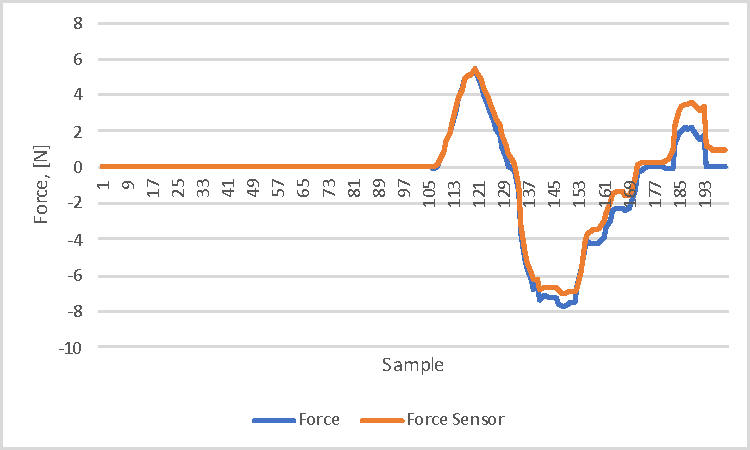
\includegraphics[width=100mm]{fig/results/syst_error.pdf}
	\end{center}
	\vspace{-4mm}
	\caption[Actual and Measured Forces in X-direction]
	{Actual and Measured Forces in X-direction}
	\label{fig:Syst_err}
	\vspace{-2mm}
\end{figure}

Another issue with the mechanical design can be seen from Figure

\begin{figure}[h]
	\begin{center}
	\includegraphics[width=100mm]{fig/results/device_bottom.png}
	\end{center}
	\vspace{-4mm}
	\caption[Y-direction Thickness of the Sensor]
	{Y-direction Thickness of the Sensor}
	\label{fig:Syst_err}
	\vspace{-2mm}
\end{figure}

	Comparison of two Z-component of the force measurement methods have shown, that Z Device has lower 
	
We tried to measure force in Z-direction, but unfortunately results shown that developed system was not accurate and sensitive enough. To improve system we can suggest to change strain gauges to more sensitive ones. Since we have small room for deformation - around 0.3 mm, we can not afford more deformation by using thinner or longer plates. Therefore, we decided to use motor current readings for z-directional reading of the force.

The force-sensing devices were designed so they can easily fit the daVinci cannula and the sterile adapter. The tolerances are compensated by adjustment of the set screws.

The system has separate wheatstone bridges for each direction, giving the ability to measure each component of the force independently. However, Z Device and X-Y device cannot work together at the same time, because created X-Y device takes the Z-component of the force and slightly restricts rotation of the shaft. In order to solve that issue, we can change mechanical design of the X-Y device by increasing the size of the sleeve and adding slippery material between the shaft and the sleeve (Figure \ref{fig:NewXYDesign}). However, it will cause other issues with increased incision size to 1.9 cm. Usually size of the incision should be in range 1-2 cm \cite{_laparoscopy}. It will be still in appropriate range, however the recovery time would increase. Another option could be moving the X-Y device on the top of cannula or changing the cannula design and applying sensors on it.

\begin{figure}[h]
	\begin{center}
		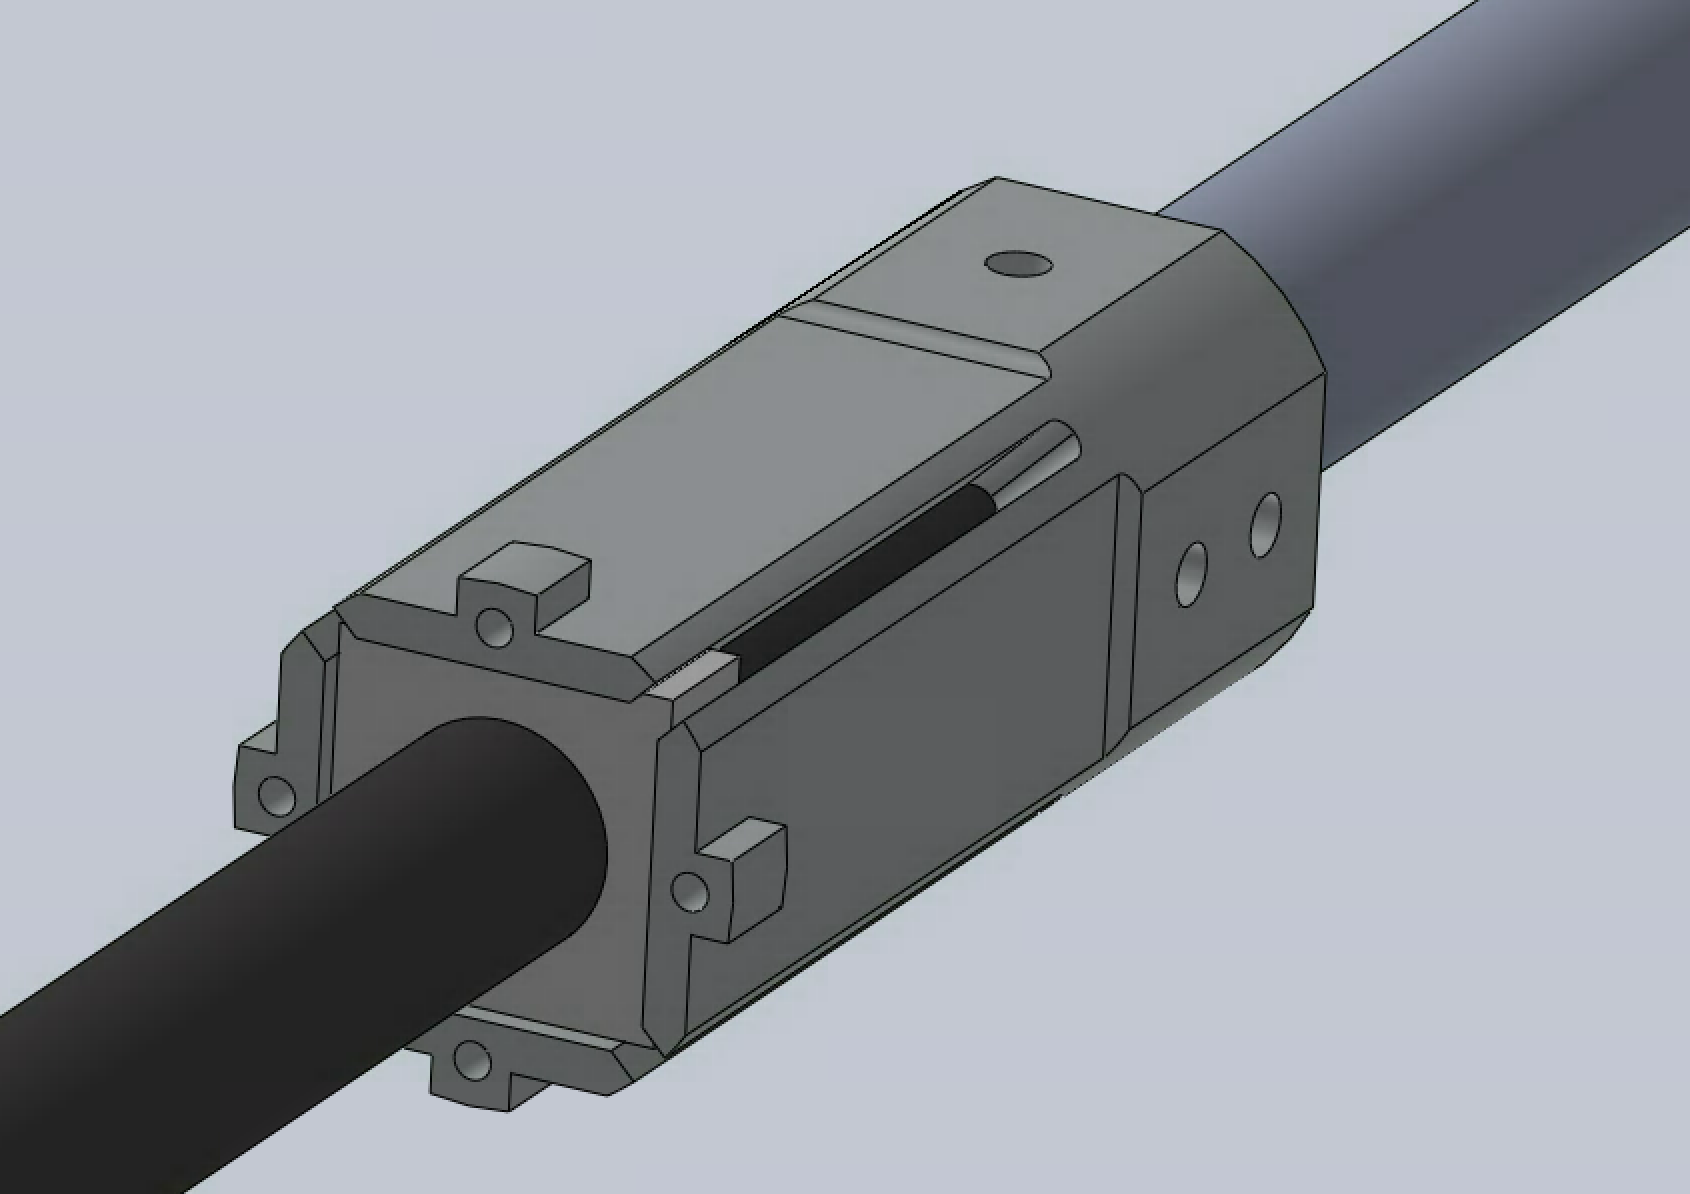
\includegraphics[width=120mm]{fig/methods/new_xy_dev.png}
	\end{center}
	\vspace{-4mm}
	\caption[New X-Y Device Design]
	{New X-Y Device Design}
	\label{fig:NewXYDesign}
	\vspace{-2mm}
\end{figure}
	
	Both devices should undergo sterilization. One of the devices goes inside the patient, meaning that it should be created using biocompatible materials. Current version of the device is not biocompatible. We can achieve biocompatibilty by using Stainless Steel as a device material and biocompatible epoxy to cover strain gauges, also teflon coated wires should be used for all electrical connections. Use of stainless steel will require change of the device dimensions, since the material has different elasticity. Also, epoxy cover can alter readings results.
	
	The real-time haptic feedback requires minimum data acquisition speed to be 1 kHz \cite{seungmoon_choi_effect_2004}. However, the current maximum speed is 588 Hz due to limitation of data transfers speed using serial communication with computer (115.2 Kbps). In order to increase the speed, we can change the communication channel to SPI (up to 10 Mbps) \cite{_uart_porotocol} or one of the wireless protocols, such as Bluetooth (up tp 1 Mbps) or wifi (up to 100 Mbps) \cite{_wireless_protocols}. Also, communication protocol between microcontroller and ADC can be changed from SPI to faster parallel communication. Additionally, the microcontroller can be changed to faster one, so it can support wireless communication. All these changes require change of the PCB design and microcontroller software. Also, in the PCB the amount of Wheatstone bridges and ADCs should be increased from 2 to 4 to reduce the overall size of the system by removing second PCB and master-slave communication.
	
	Another thing that could be changed is type of sensor. Use of QTC-pills seem to be promising approach, since it has smaller size and higher sensitivity. However, it has nonlinear output, meaning some electrical design and calibration complications.
	
Other disadvantages of the system are addition of the cost to already expensive system and biocompaitibily and sterilization issues. Also addition of the weight to the arm could alter robot performance. Taking into account, that the device will be placed close to the center of rotation of the robot arm, it will have minimal affect on the moment of inertia in comparison to sensors added to the grippers.

%Some of the requirements for the devices were met, such as sensitivity, resolution, force measurement range, signal-to-noise ratio. However, the system has some major drawbacks due to high hysteresis and errors.

The created sensor gives 3-DOF force feedback. Showing that it is possible to add force-feedback in the daVInci robot without major changes of the existing system. However, not all of the requirements for the force measuring system were satisfied, meaning that the sensors need further improvements in both electrical and mechanical designs.